
%(BEGIN_QUESTION)
% Copyright 2011, Tony R. Kuphaldt, released under the Creative Commons Attribution License (v 1.0)
% This means you may do almost anything with this work of mine, so long as you give me proper credit

Examine these two control ``loops'' (transmitter-controller-valve systems) for an industrial boiler, controlling both water level and steam pressure:

$$\includegraphics[width=15.5cm]{i01688x01.eps}$$

If the PIC setpoint is 225 PSI and the measured steam pressure begins to rise above that value, how should the PIC respond, and how will this response bring the steam pressure back down to setpoint?

\vskip 10pt

Describe a situation where the {\it block} and {\it bypass} hand valves installed on the fuel gas line might ever be used, either by operations or by maintenance personnel.

\vskip 10pt

If the I/P transducer on the level control loop suddenly fell out of calibration in such a way that it output a pneumatic signal that was too low, how would this affect the control of water level in the steam drum?

\filbreak

\vskip 20pt \vbox{\hrule \hbox{\strut \vrule{} {\bf Suggestions for Socratic discussion} \vrule} \hrule}

\begin{itemize}
\item{} Explain what would happen to this process if the air supply to the feedwater valve's I/P transducer failed.
\item{} Explain what would happen to this process if the air supply to the fuel valve's I/P transducer failed.
\item{} Explain how both control loops will respond to a sudden increase in steam demand.
\end{itemize}

\underbar{file i01688}
%(END_QUESTION)





%(BEGIN_ANSWER)

If steam pressure begins to fall below setpoint, the PIC should send a decreasing signal to the fuel gas valve, causing the burner to output less heat and thereby lowering the steam pressure to setpoint again.  If well-tuned, a loop controller will drive its output signal to {\it whatever value is necessary} to achieve PV = SP.

\vskip 10pt

The manual block and bypass valves are useful for taking the fuel control valve out of service while the boiler is still running.  This allows technicians to stroke-test and even replace the control valve without shutting down the boiler.  I will let you describe and explain the sequence of valve motions necessary to take a working control valve out of service.

\vskip 10pt

A falsely-low pressure signal coming from the I/P might cause the actual water level to {\it drop} if the change was sudden, but the LIC will eventually compensate for this change by adjusting its output signal value until the control valve is at the correct position again.

%(END_ANSWER)





%(BEGIN_NOTES)

It is possible that a calibration error in the I/P could permanently affect water drum level, but only if that calibration error were so severe that the controller could not get the valve to the correct position even with its output signal saturated (i.e. $\geq$ 20 mA or $\leq$ 4 mA).

%INDEX% Basics, control loop troubleshooting: determining effect of specified fault(s)

%(END_NOTES)


